Dans les chapitres précédants, les bases théoriques sur les automates et langages ont été posées. Celles-ci ont été suivies de concepts plus étroitement liés à LeVer tels que les automates à files, les traces, traces annotées et langages associés. Un dernier élément présenté dans la section \ref{sec:unsafe} est la sécurité d'un état ou d'un automate.

En appliquant l'algorithme d'Angluin \cite{Angluin87} selon la méthode LeVer \cite{Vardhan04}, il est possible de se prononcer sur la sécurité pour toute une classe d'automates à files : ceux pour lesquels le language de traces annotées est régulier.

L'objectif dès lors n'est pas d'apprendre le language de l'automate à file mais le language de trace associé, et d'adapter la méthode pour répondre à la question de sécurité. En formulant les bonnes propriétés, il est également possible d'interrompre l'algorithme d'apprentissage avant terme si l'on peut se prononcer sur la sécurité de façon certaine.


\begin{figure}[H]
	\centering

	\resizebox{\textwidth}{!}{
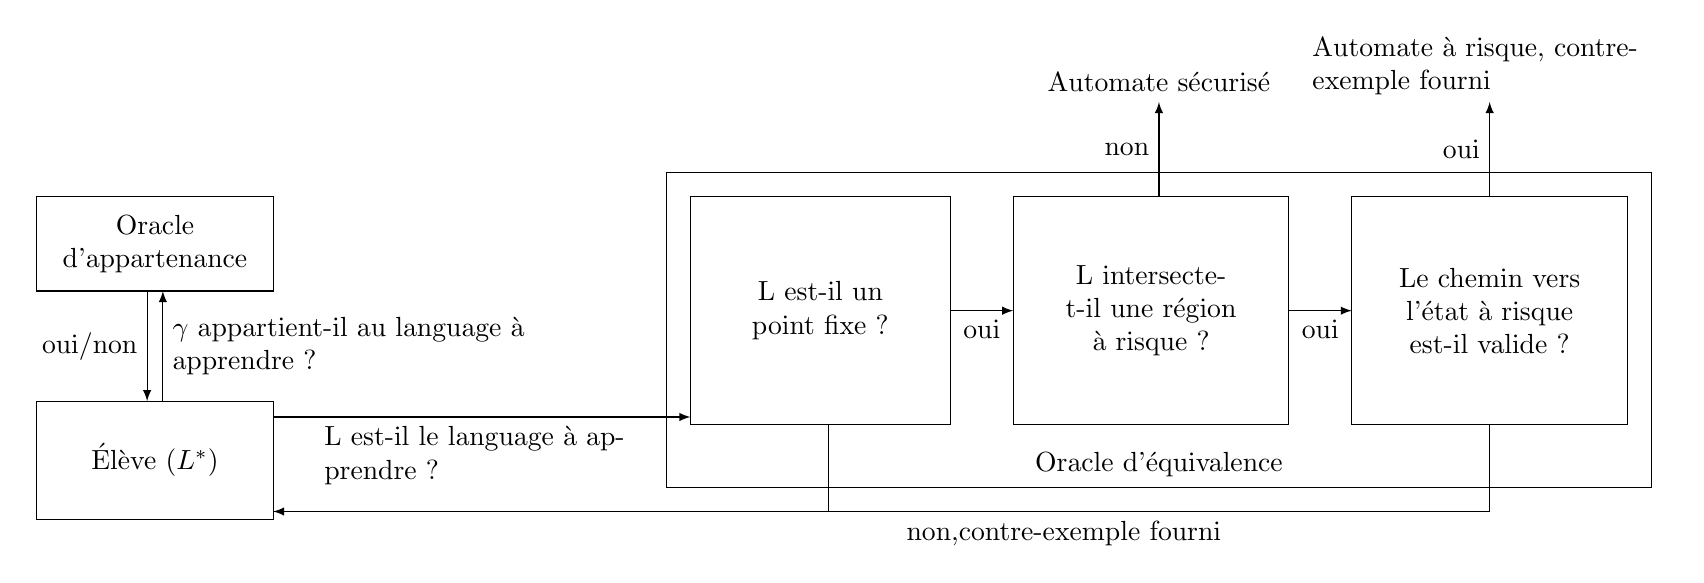
\begin{tikzpicture}
	\tikzset{>=latex}

  \draw (-3,-2.9) rectangle (0,-4.4) node[pos=.5] {Élève ($L^*$)};
  \draw (5,0) rectangle (17.5,-4);
	\draw[->] (0,-3.1) -- (5.3,-3.1) node[pos=0.5,below,text width=4cm] {L est-il le language à apprendre ?};

  \draw (-3,-0.3) rectangle (0,-1.5) node[pos=.5,text width=3cm,align=center] {Oracle\\ d'appartenance};
  \draw[->] (-1.4,-2.9) -- (-1.4,-1.5) node[pos=0.5,right,text width=5cm] {$\gamma$ appartient-il au language à apprendre ?};
  \draw[<-] (-1.6,-2.9) -- (-1.6,-1.5) node[pos=0.5,left] {oui/non};

  \node[draw=none] at (11.25, -3.7) {Oracle d'équivalence};

  \draw (5.3, -0.3) rectangle (8.6, -3.2) node[pos=0.5,text width=3cm,align=center] {L est-il un point fixe ?};
  \draw (9.4, -0.3) rectangle (12.9, -3.2) node[pos=0.5,text width=3cm,align=center] {L intersecte-t-il une région à risque ?};
  \draw (13.7, -0.3) rectangle (17.2, -3.2) node[pos=0.5,text width=3cm,align=center] {Le chemin vers l'état à risque est-il valide ?};

  \draw[->] (8.6, -1.75) -- (9.4,-1.75) node[pos=0.5,below] {oui};
  \draw[->] (12.9, -1.75) -- (13.7,-1.75) node[pos=0.5,below] {oui};
  \draw[->] (15.45, -4.3) -- (0, -4.3) node[pos=0.35,below] {non,contre-exemple fourni};
  \draw[-] (7.05, -3.2) -- (7.05, -4.3);
  \draw[-] (15.45, -3.2) -- (15.45, -4.3);

	\draw[->] (11.25,-0.3) -- (11.25,0.9)node[pos=0.5,left] {non};
	\draw[->] (15.45,-0.3) -- (15.45,0.9)node[pos=0.5,left] {oui};

	\node[draw=none] at (11.25, 1.15) {Automate sécurisé};
	\node[draw=none,text width=4.5cm] at (15.45, 1.36) {Automate à risque, contre-exemple fourni};


\end{tikzpicture}
}
\caption{Vue schématique de l'algorithme d'Angluin pour LeVer\cite{Vardhan04}}

\end{figure}

Contrairement à la version proposée dans la section \ref{sec:angluin}, ici il n'est pas possible de tester directement l'équivalence entre $L$ et le language à apprendre. En effet, ce dernier peut ne pas être régulier et de façon générale le professeur ne connaît justement pas l'automate permettant une telle comparaison si celle-ci existe.

Ici, le professeur passe par trois questions mais à aucun moment il sait dire si $L$ est exactement le language à apprendre. Il peut soit se prononcer sur la sécurité, soit dire avec certitude qu'il existe une meilleure approximation.

\begin{itemize}
	\item \emph{L est-il un point fixe ?} Cette question fait référence à l'application de la fonction d'extension de trace de la section \ref{ss:extension}.
	\item \emph{L intersecte-t-il une région à risque ?} Si $L$ est un point fixe de $\mathcal{F}$, il est soit le language à apprendre soit un point fixe le contenant. Si une surapproximation n'a pas d'intersection avec une région à risque, $L$ n'en a pas non plus.
	\item \emph{Le chemin vers l'état à risque est-il valide ?} Si un \emph{chemin à risque} (menant à un état à risque) existe dans $L$, est-il valide ? C'est-à-dire, appartient-il au language visé et représente-t-il bien un chemin dans l'automate à files étudié ?
\end{itemize}

Les prochaines sections décrivent ce nouvel oracle d'appartenance et celui d'équivalence avec les trois questions posées avant de revenir sur une vue d'ensemble. De la sorte, la section \ref{sec:global} résume quand et pourquoi cette méthode fonctionne.
